\section{Formulation}
\label{sec:formulation}
Following the formulation of general history-dependent given by (\ref{eq:generalFric}), 
we still further assume that the dependence on the slip history can be modeled as dependence on hidden variables $\bm{\xi} \in \mathbb{R}^d$. 
We introduce three potentials, 
$W(x)$, 
$D^\dagger(\dot{x}, \bm{\xi})$ and $D(\dot{\bm{\xi}})$, 
whose derivatives give rise to the friction coefficient and evolution law of $\bm{\xi}$, i.e., 
\begin{align}
    &f^{P}(\dot{x}, \boldsymbol{\xi}) = \frac{d W}{d x}(x) + \frac{\partial D^\dagger}{\partial \dot{x}}(\dot{x}, \bm{\xi}) \label{eq:fpot}, \\
    &\frac{d D}{d \dot{\boldsymbol{\xi}}}(\dot{\bm{\xi}}) + \frac{\partial D^\dagger}{\partial \boldsymbol{\xi}}(\dot{x}, \bm{\xi}) = 0 \label{eq:evolutionXi},  
\end{align}
where $f^{P}$ is the potential formulation friction coefficient.  
$x$ is local slip and $V = \dot{x}$ is local slip rate, 
$\bm{\xi} \in \mathbb{R}$ is a $d$ dimensional vector of internal variables that encodes the local slip history. 

The advantage of this potential formulation is that the solution of an incremental problem with such friction are equivalent to the stationary point of a scalar function $J(x, \bm{\xi})$. Take an example of the spring slider configuration under displacement-control as shown in Figure~\ref{fig:springslider}. 
The system is driven by prescribing $x_p(t)$, 
and the force of the spring is linearly dependent on its elongation with spring constant $k$. 
There is history-dependent friction between the mass block and the ground, 
gravity acceleration is $g$. 
Assuming that the history-dependent friction can be represented in the above potential form, 
the equations of motion of the system is 
\begin{align}
    m\Ddot{x} - k(x_p(t) - x(t)) + mg \left(\frac{d W}{d x} + \frac{\partial D^\dagger}{\partial \dot{x}}\right)&= 0 \label{eq:springsliderEOM1} \\
    \frac{d D}{d \dot{\boldsymbol{\xi}}}(\dot{\bm{\xi}}) + \frac{\partial D^\dagger}{\partial \boldsymbol{\xi}}(\dot{x}, \bm{\xi}) &= 0 \notag. 
\end{align}
Given the solution at current time $x_n, \bm{\xi}_n$, 
and the time increment $\Delta t = t_{n+1} - t_n$, 
define 
\begin{align}
    E^{sp}(x) &= \frac{1}{2}\left(x(t) - x_p(t)\right)^2 \label{eq:Esp} \\
    E^{in}(x) &= \frac{1}{2}\left(\frac{x - 2 x_n + x_{n-1}}{\Delta t}\right)^2 \label{eq:Ein}, 
\end{align}
as the spring potential and the inertia potential, 
and
\begin{align}
    J(x, \bm{\xi}; \Delta t, x_n, \bm{\xi}_n) &= E^{sp}(x) + E^{in}(x) + W(x) + \Delta t D^\dagger\left(\frac{x - x_n}{\Delta t}, \bm{\xi}\right) + \Delta t^2 D\left(\frac{\bm{\xi} - \bm{\xi}_n}{\Delta t}\right) \label{eq:Jfunctional}
\end{align}
as the system potential. 
Then it is straight-forward too see that the backward Euler implicit update is
\begin{align}
    x_{n+1}, \bm{\xi}_{n+1} &= \argmin_{x, \bm{\xi}} J(x, \bm{\xi}; \Delta t, x_n, \bm{\xi}_{n}) \label{eq:JfunctionalMin}. 
\end{align}
This is well-posed if $J$ is convex in $(x, \bm{\xi})$. 
Convexity of $J$ is trivial if $W, D^\dagger, D$ are all convex in $(x, \bm{\xi})$. 
However, 
usually not all of $W, D^\dagger, D$ are convex, 
especially $D^{\dagger}$, 
since if friction coefficient decreases with slip rate, 
i.e., 
\begin{align}
    \frac{\partial f}{\partial \dot{x}} = \frac{\partial^2D^\dagger}{\partial \dot{x}^2} < 0 \label{eq:nonConvexDdagger}. 
\end{align}
In such cases, 
one needs to adjust $\Delta t$ such that $E^{in}$ dominates and $J$ is convex. 

\begin{figure}
    \centering
    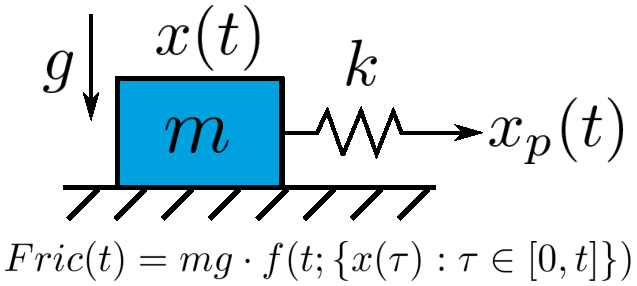
\includegraphics[width=0.4\textwidth]{figures/SpringSlider.pdf}
    \caption{Example: spring slider under displacement-control driving force}
    \label{fig:springslider}
\end{figure}

In summary, 
by developing such a potential formulated friction, 
the implicit solving process of dynamic problems are turned into a convex optimization problem, 
which would guarantee us the existence of a unique solution for $(x_{n+1}, \bm{\xi}_{n+1})$. 
This would facilitate implicit solution which is usually difficult with the original rate-and-state friction. 
Since the original rate-and-state friction given by (\ref{eq:fRS}) is able to fit experimental data well with 4 parameters, 
it is crucial to verify that the potential-formulated friction specified by (\ref{eq:fpot}) can replicate rate-and-state friction sequences, 
with some selected $W, D^\dagger$ and $D$. 

In practice, 
it is useful to work with the dual formulation. 
Let $D^*(\bm{\dot{d}})$ be the Legendre transform of $D(\bm{\dot{\xi}})$, 
\begin{align}
    D^*\left(\dot{\bm{d}}\right) &= \sup_{\bm{\dot{\xi}} \in \mathbb{R}^d} \left\{\la \bm{\dot{d}}, \bm{\dot{\xi}} \ra -D(\dot{\bm{\xi}})\right\}. \label{eq:LegendreDstar}
\end{align} 
The advantage of using $D^*$ instead of $D$ is that instead of solving the non-linear equation for $\dot{\bm{\xi}}$ given by (\ref{eq:evolutionXi}), 
it is equivalent to computing $\dot{\bm{\xi}}$ by 
\begin{align}
    \dot{\bm{\xi}} &= \frac{d \Tilde{D}^*}{d \dot{\bm{d}}}\left(-\frac{\partial \Tilde{D}^\dagger}{\partial \bm{\xi}}\right) \label{eq:ComputeXiDot}, 
\end{align}
if $D\left(\bm{\dot{\xi}}\right)$ is convex in $\bm{\dot{\xi}}$. 


\section{Neural Network and training}
\label{sec:NN}
We use Neural Networks to approximate the above potentials within the deeping learning environment PyTorch \cite{paszke2019pytorch}, i.e., 
\begin{align}
    W(x) \approx W_{NN}(x; w_W), 
    D^\dagger(\dot{x}, \bm{\xi}) \approx D^\dagger_{NN}(\dot{x}, \bm{\xi}; w_{D^\dagger}), 
    D^*\left(\dot{\bm{d}}\right) \approx D^*_{NN}\left(\dot{\bm{d}}, w_{D^*}\right)\label{eq:NNpotentials},  
\end{align}
and we call the resulting architecture a Recurrent Neural Operator (RNO) following \cite{BurigedeEric2023, BurigedeMarkovian2023}. 

To find proper $W, D^\dagger$ and $D$ that give $f^{NN}$ similar enough to $f^{RS}$ under a set of rate-and-state parameters, 
we generate a synthetic dataset of $f^{RS}$'s by prescribing the slip histories $\{V = \dot{x}(t) : t \in [0, T]\}$. 
We then fit $f^{NN}$'s to $f^{RS}$'s by optimizing over the parameters of $W_{NN}, D^\dagger_{NN}$ and $D_{NN}$, 
as shown in Figure~\ref{fig:training}. 
\begin{figure}
    \centering
    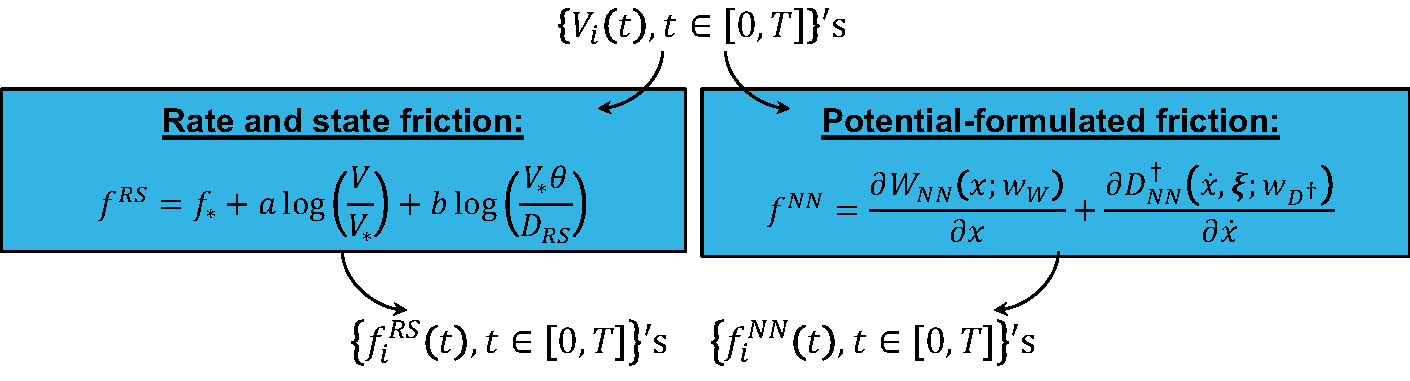
\includegraphics[width=0.8\textwidth]{figures/training.pdf}
    \caption{Training of $W, D^\dagger$ and $D$ through fitting $f^{NN}$ to $f^{RS}$}
    \label{fig:training}
\end{figure}
And the loss function we use for training of the potentials is relative $L_p$ error, 
i.e., 
\begin{align}
    w_W^*, w_{D^\dagger}^*, w_D^* = \argmin_{w_W, w_{D^\dagger}, w_D} \frac{1}{N} \sum_{i=1}^N \frac{\|f^{NN}_i(t) - f^{RS}_i(t)\|_{L_p}}{\|f^{RS}_i(t)\|_{L_p}} \label{eq:relativeLpError}. 
\end{align}
In this study, 
the rate-and-state friction parameters are chosen to be 
\begin{align*}
    a &= 0.011, \\
    b &= 0.016, \\
    D_{RS} &= 0.01, \\
    f_* &= 0.58, 
\end{align*}
such that we do examine the ability of potential formulated friction to fit rate-weakening ($a - b < 0$) rate-and-state friction, 
which is more challenging to solve  numerically. 
Regarding the specific choices of $V_i(t)$'s, 
we take inspiration from both velocity jump tests for rate-and-state friction \cite{ruina_slip_1983}, 
as well as continuous variation sequences from the previous studies of RNO \cite{BurigedeEric2023, BurigedeMarkovian2023}. 
For the velocity jump sequences, 
$V_i(t)$'s are simple functions, 
i.e., the sum of a finite number of Heaviside functions, 
as shown by the first example in Figure~{\ref{fig:19thAnd99thRS}}. 
Note that the prescribed velocity jumps have to be on the log scale to cause significant changes in $f^{RS}$.  
While for the continuous variation sequences, 
$V_i(t)$'s vary continuously with $t$ and change their monotonicity at randomly-sampled times, 
as shown by the second example in Figure~\ref{fig:19thAnd99thRS}. 
\begin{figure}
    \centering
    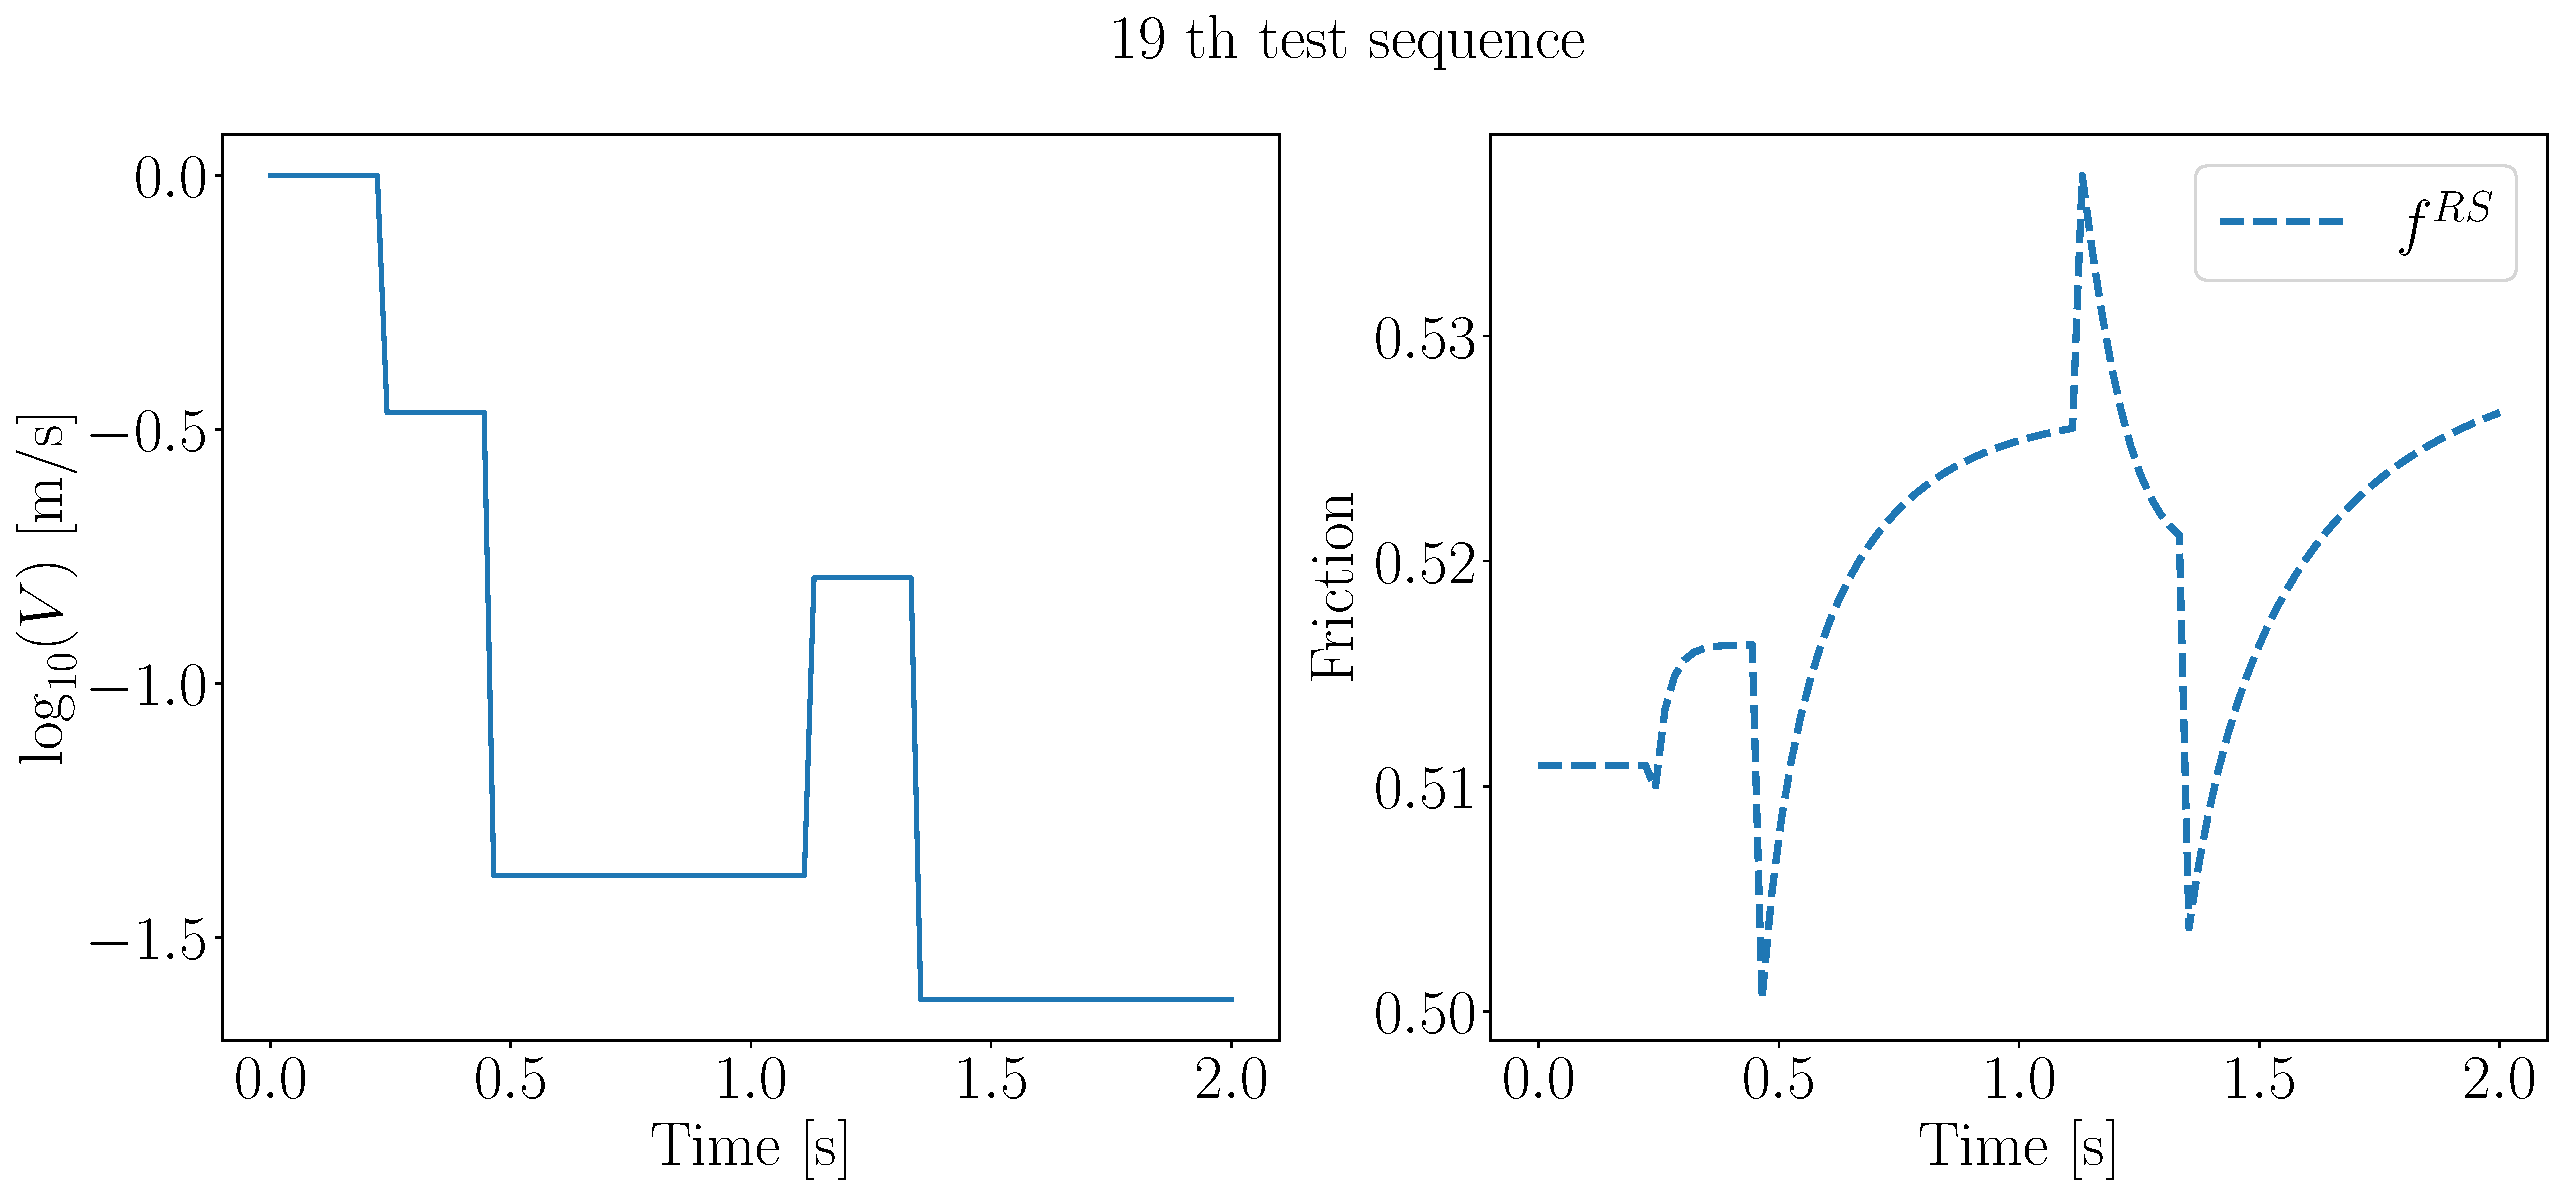
\includegraphics[height=0.3\textheight]{figures/19thRS.pdf}
    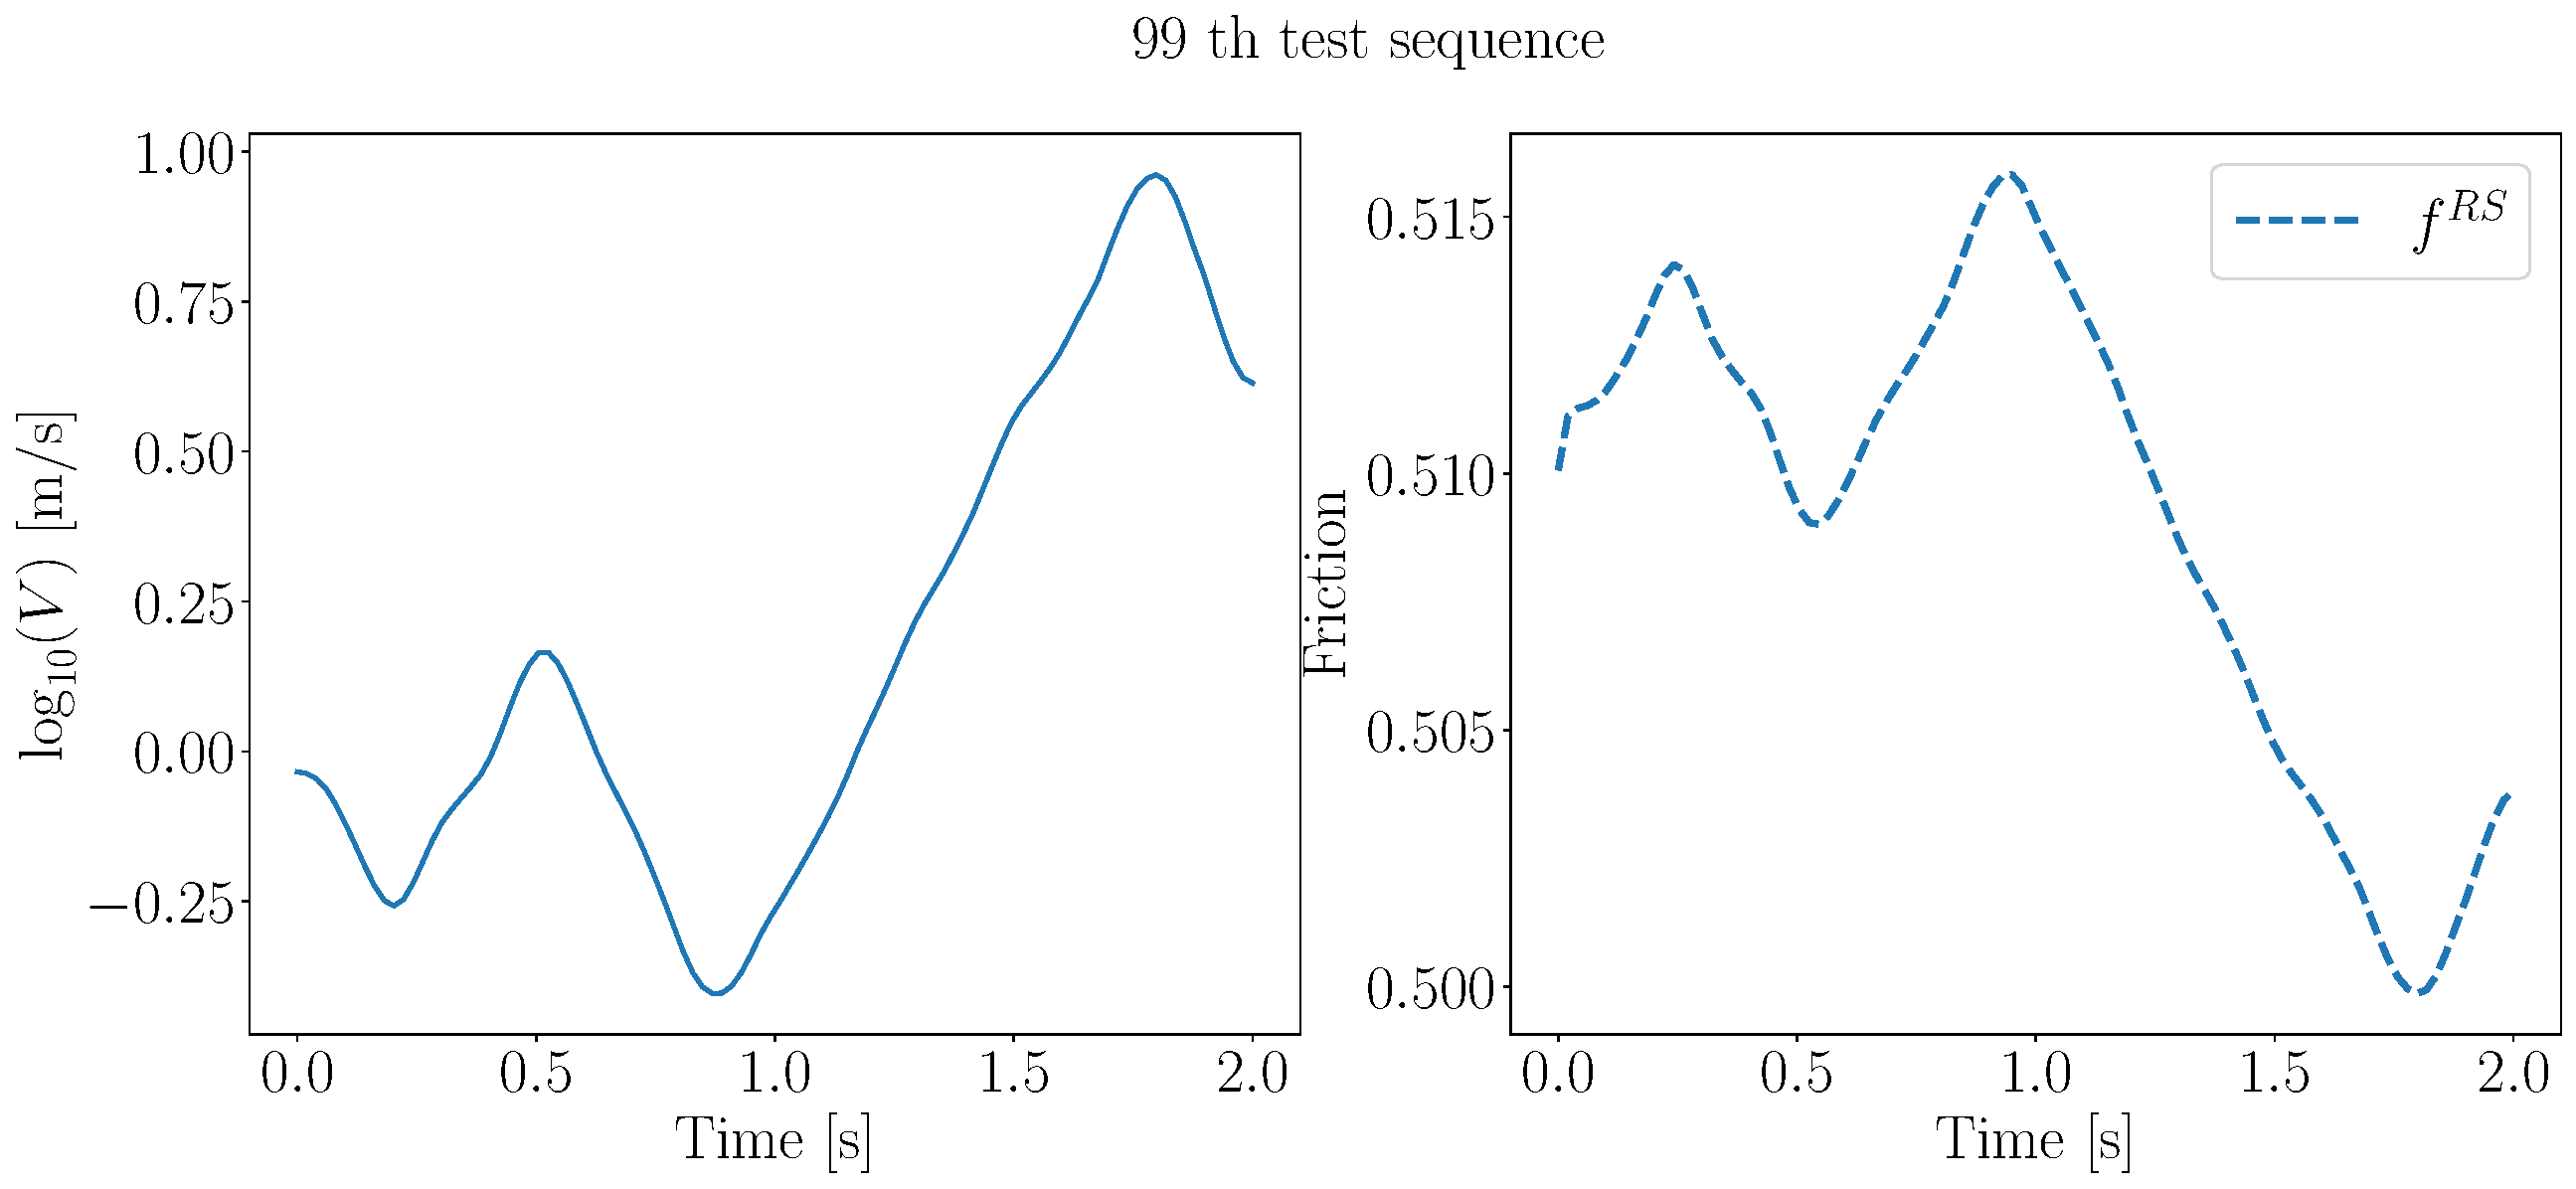
\includegraphics[height=0.3\textheight]{figures/99thRS.pdf}
    \caption{Examples of velocity jump $V_i(t)$ (upper, sequence 19), 
    continuous variation $V_i(t)$ (lower, sequence 99) and their corresponding $f^{RS}$s in the synthetic dataset.}
    \label{fig:19thAnd99thRS}
\end{figure}

Within the training process, 
we apply Optuna \cite{akiba2019optuna} optimization package for hyper-parameter tuning of the Recurrent Neural Operators (RNO). 
Those hyper-parameters include learning rate, 
depth of the Neural Network, 
number of neurons within each layer, 
$p$ value for the $L_p$ norm, 
as well as the batch size in the training dataset. 
Detailed algorithm regarding the training process can be found in Algorithm~\ref{alg:TrainingOneEpoch}. 

\begin{algorithm}[H]
\caption{Training $W_{NN}(x; w_W), D_{NN}^\dagger(\dot{x}, \bm{\xi}; w_{D^\dagger})$ and $D_{NN}^*(\dot{\bm{d}}; w_D)$}\label{alg:TrainingOneEpoch}
\begin{algorithmic}
%% Setting parameters
% Input space
\Require training sequences $\left\{\dot{x}_i = V_{i}(t), f^{RS}_i(t) : t \in [0, T]\right\}_{i = 0}^N$.  
\Require $N_{epochs}$
%% Algorithm begins
\State $epoch = 0$
\While{$epoch<N_{epochs}$}
    \For {$i \in \{0, 1, ..., N\}$} \Comment{In practical sequences are passed in batches.}
        \State Fix $w_W$, $w_{D^\dagger}$, $w_D$
        \For {$n = 1, 2, ..., N^{(i)}$} \Comment{$N^{(i)}$ is number of time steps of sequence $i$. }
            \State $\xi_n \gets \xi_{n-1} + (t_n-t_{n-1}) \dot{\bm{\xi}}_{n-1}$
            \State $f^{NN}_n \gets \frac{\partial W_{NN}}{\partial x}(x_n) + \frac{\partial D^\dagger_NN}{\partial \dot{x}}(\dot{x}_n, \bm{\xi}_n)$
            \State \textcolor{red}{$\bm{\dot{\xi}}_n \gets $ solution of $\frac{d D_{NN}}{d \dot{\boldsymbol{\xi}}}(\dot{\bm{\xi}}) + \frac{\partial D_{NN}^\dagger}{\partial \boldsymbol{\xi}}(\dot{x}_n, \bm{\xi}_n) = 0$}
            \Comment{In practical $\dot{\bm{\xi}}_n = \frac{d D_{NN}^*}{d \dot{\bm{d}}}\left(-\frac{\partial D_{NN}^\dagger}{\partial \bm{\xi}}\left(\dot{x}_n, \bm{\xi}_n\right)\right)$}
        \EndFor
        \State Compute Loss $L(w_W, w_{D^\dagger}, w_D) = \|f^{RS} - f^{NN}(w_W, w_{D^\dagger}, w_D)\|_{{L}^p} / \|f^{RS}\|_{{L}^p}$
        \State Update $w_W, w_{D^\dagger}, w_D$ based on the gradient of $L$ w.r.t. $w_W, w_{D^\dagger}, w_D$
    \EndFor
    \State $epoch \gets epoch+1$
\EndWhile
\end{algorithmic}
\end{algorithm}